% Incluyendo el preambulo de LaTeX para configurar los paquetes que se vayan usando
% Configuracion inicial del documento
\documentclass[a4paper]{article}

% Paquetes utilizados
\usepackage[utf8]{inputenc}
\usepackage[spanish, es-tabla]{babel}
\usepackage{float}
\usepackage{graphicx}
\usepackage{multirow}
\usepackage{circuitikz}

% Paquetes de matematica
\usepackage{amsmath}
\usepackage{amssymb}
\usepackage{steinmetz}

% Paquetes para excel
\usepackage{csvsimple}

% Configuracion del informe
\setlength{\parindent}{0pt}
\setcounter{secnumdepth}{0}

\usepackage[a4paper, 
    includehead, 
    footskip=7mm, 
    headsep=6mm, 
    headheight=4.8mm,
    top=25mm, bottom=25mm, left=25mm, right=25mm]{geometry}

\usepackage{hyperref}
\hypersetup{
    colorlinks=true,
    linkcolor=blue,
    filecolor=magenta,      
    urlcolor=blue,
    citecolor=blue,    
}

% Abrir y crear el documento, llamar a cada uno de los ejercicios
\begin{document}

    % Crear y configurar el titulo/caratula del informe
    \title{
        \normalfont \normalsize \textsc{Instituto Tecnol\'ogico de Buenos Aires} \\ [25pt]
        \huge Trabajo Pr\'actico Nº 3 \\
        \author{
            \\Grupo 1:\\\\Galdeman, Agust\'in Ignacio\\Gaytan, Joaqu\'in Oscar\\Kammann, Lucas Agust\'in\\Maselli, Carlos Javier\\ \\ \\ \\
            Profesores: \\\\ Cossutta, Pablo Mart\'in\\Weill, Mar\'ia Alejandra\\Salvati, Mat\'ias Dami\'an \\ \\ \\ 
        } 
        \text{Laboratorio de Electr\'onica - 2019}
    }
    \pagenumbering{arabic}

    \maketitle
    \newpage

    % Crear indice del informe
    \tableofcontents

    % Incluyendo los ejercicios realizados
    \newpage
    \section{Circuito Convertidor Boost}
El objetivo de este trabajo es realizar un conjunto de mediciones sobre el circuito ilustrado en la Fig. \ref{fig:circuito}
al cual se denomina Convertidor Boost. Cualitativamente, el funcionamiento de dicho circuito consiste en la utilizaci\'on de un transistor como dispositivo de conmutaci\'on
para abrir y cerrar la respectiva rama del circuito, de esta forma cuando el mismo se encuentra en el modo de saturaci\'on circula sobre el inductor una corriente y comienza a almacenar una
determinada cantidad de energ\'ia correspondiente al tiempo durante el cual se la cargue. Por otro lado cuando el transistor se encuentra en el modo de corte, el inductor se comienza a descargar
a trav\'es de los capacitores, carg\'andolos por corrientes lo cual permite elevar su nivel de tensi\'on en cada ciclo.
Finalmente, el diodo es utilizado para evitar que el capacitor se descargue por el transistor en el momento en que se pone en modo de saturaci\'on, en cuyo caso la descarga se hace del capacitor a la carga del circuito,
por tanto habr\'an peque\~nas variaciones de la tensi\'on que almacena en el tiempo el capacitor, tales variaciones ser\'an denominadas como ripple, y es uno de los aspectos a medir en este trabajo.

Por otro lado, el estado de la conmutaci\'on del transistor es controlado por un generador de funciones que provee una se\~nal cuadrada cuya tensi\'on debe ser siempre positiva para evitar sobrepasar
el valor de tensi\'on de ruptura de la juntura base-emisor. Mientras que la amplitud de dicha se\~nal de entrada es un aspecto importante para definir el estado de polarizaci\'on del transistor, su frecuencia y duty
permiten determinar el tiempo durante el cual se carga con corriente el inductor, y luego se descarga hacia el capacitor, esto \'ultimo tendr\'a una importante incidencia sobre el valor resultante de la salida y su ripple.

\begin{figure}[H]
    \centering
    \includegraphics[scale=0.5]{Recursos/circuito.png}
    \caption{Circuito convertidor boost}
    \label{fig:circuito}
\end{figure}

A continuaci\'on se describen una serie de experiencias y observaciones realizadas en el ensayo experimental del circuito. Vale mencionar,
que si bien inicialmente el circuito propuesto para el an\'alisis es el ilustrado en la Fig. \ref{fig:circuito}, en la pr\'actica se cambio la resistencia
de la carga $R_L = 100 \Omega$ para poder realizar mejor las mediciones.

\subsection{Barrido de frecuencias}
Se configura el generador de funciones con una onda cuadrada con valor de amplitud $5V$ y duty $50\%$. Luego se fija la frecuencia de la misma en $2kHz$ y luego
se va incrementando gradualmente hasta alcanzar los $200kHz$ para poder observar el comportamiento del circuito para cada frecuencias de forma aproximada. En la Fig.
\ref{fig:barrido_frecuencia} se pueden observar los resultados de cuatro de las mediciones realizadas, donde cabe destacar que la onda de color amarilla corresponde a la entrada
provista por el generador de funciones, y la verde es la salida medida sobre la $R_L$.

De estos resultados lo que se observa es que la frecuencia de la onda cuadrada que controla la conmutaci\'on del transistor, efectivamente tiene una influencia sobre el valor del ripple
de la salida, esto es, las variaciones del nivel de continua que idealmente se esperar\'ia fueran nulas. Adem\'as, para las bajas frecuencias la salida ten\'ia un valor medio aproximadamentes de $V_L = 9V$ mientras que para los casos
de mayor frecuencia el valor se fue corriendo aproximadamente hacia $V_L = 11V$.

\begin{figure}[H]
    \centering
    \begin{tabular}{c c}
        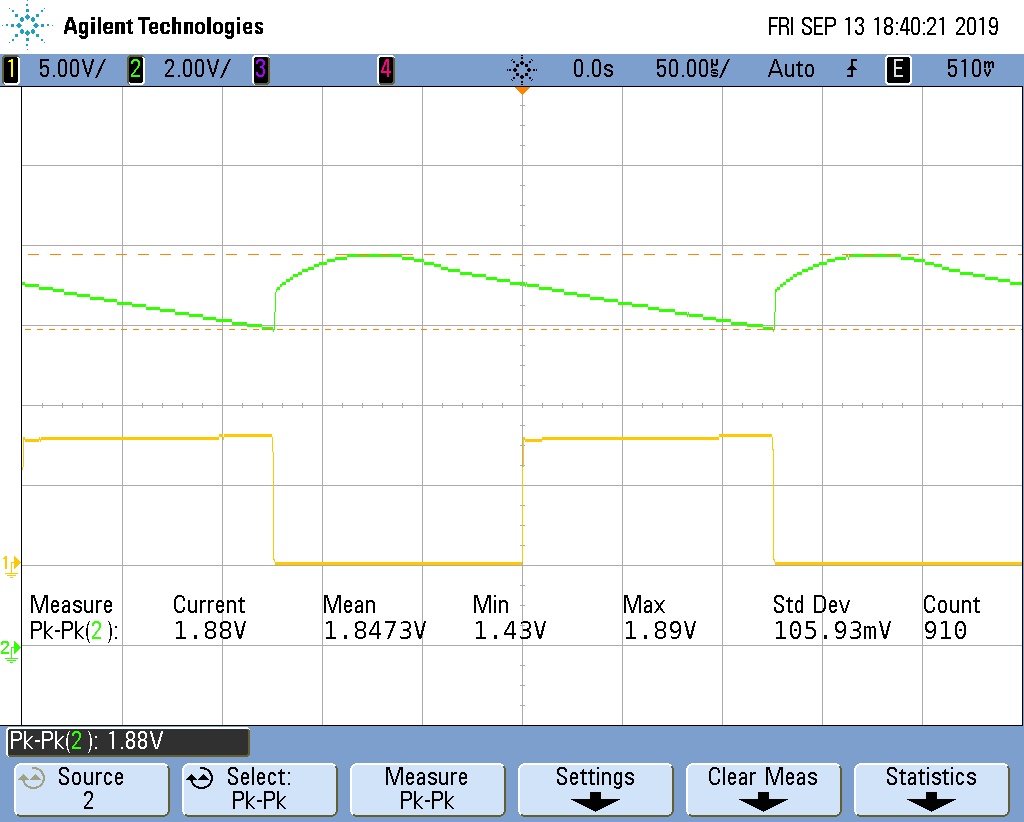
\includegraphics[scale=0.2]{../Mediciones/Osciloscopio/Barrido_Frecuencia/scope_1.png} & 
        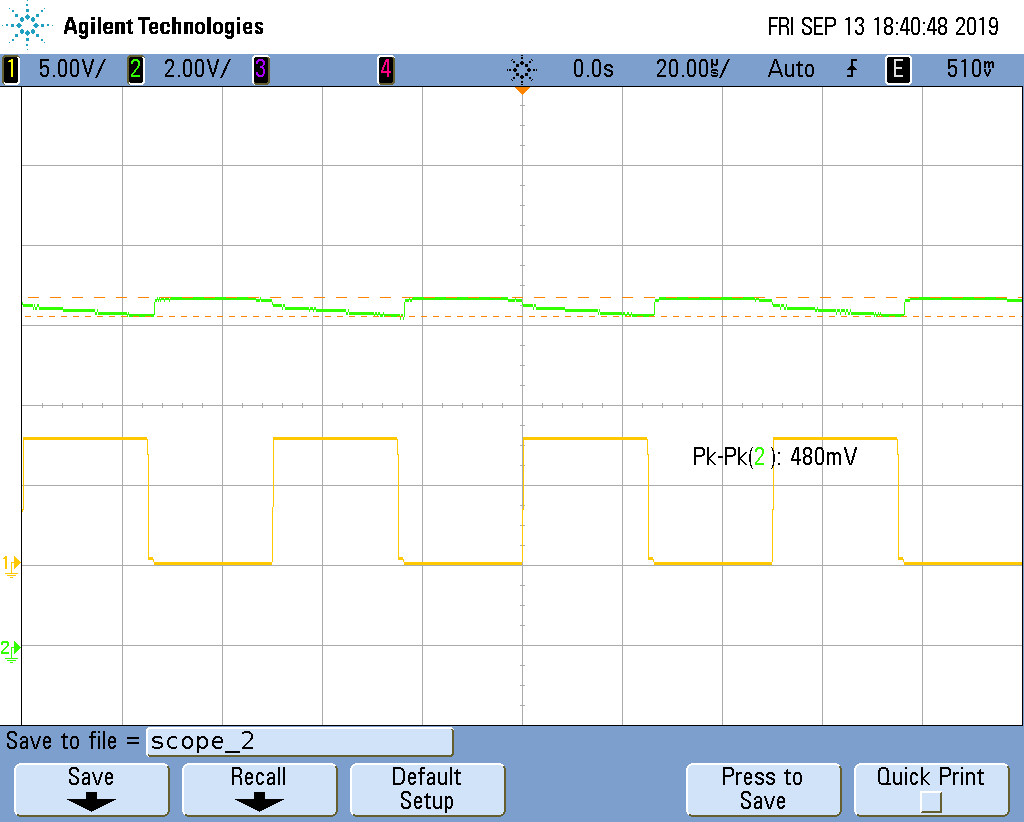
\includegraphics[scale=0.2]{../Mediciones/Osciloscopio/Barrido_Frecuencia/scope_2.png} \\
        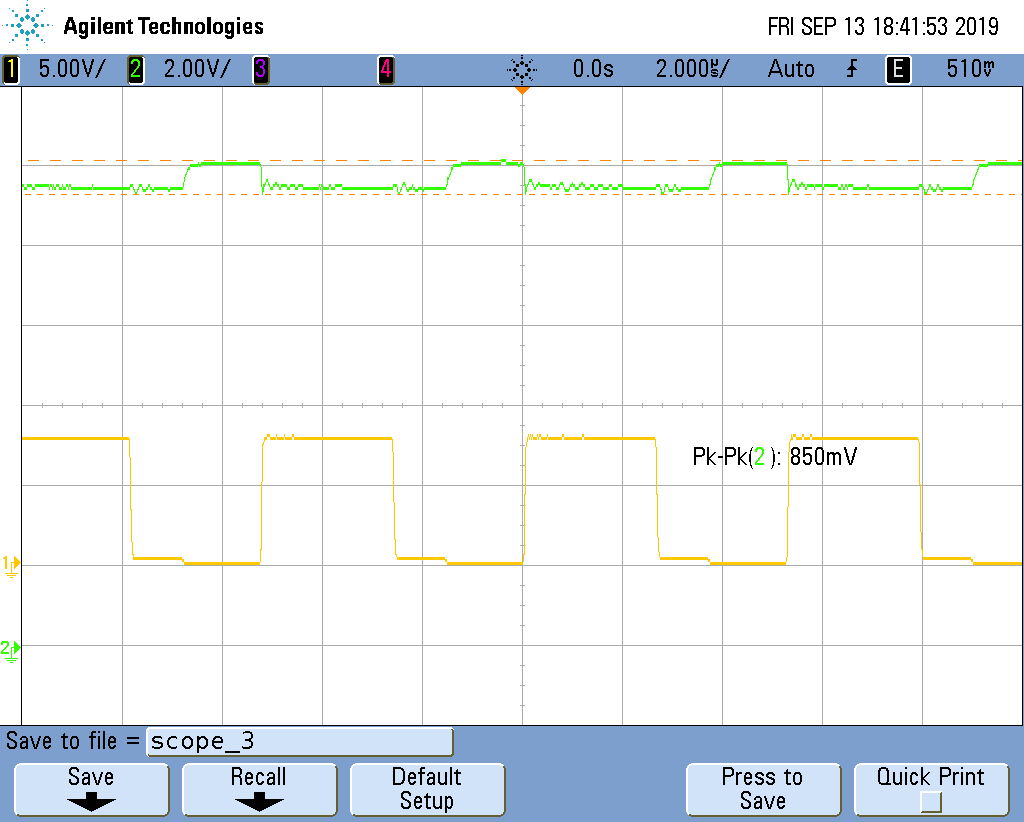
\includegraphics[scale=0.2]{../Mediciones/Osciloscopio/Barrido_Frecuencia/scope_3.png} & 
        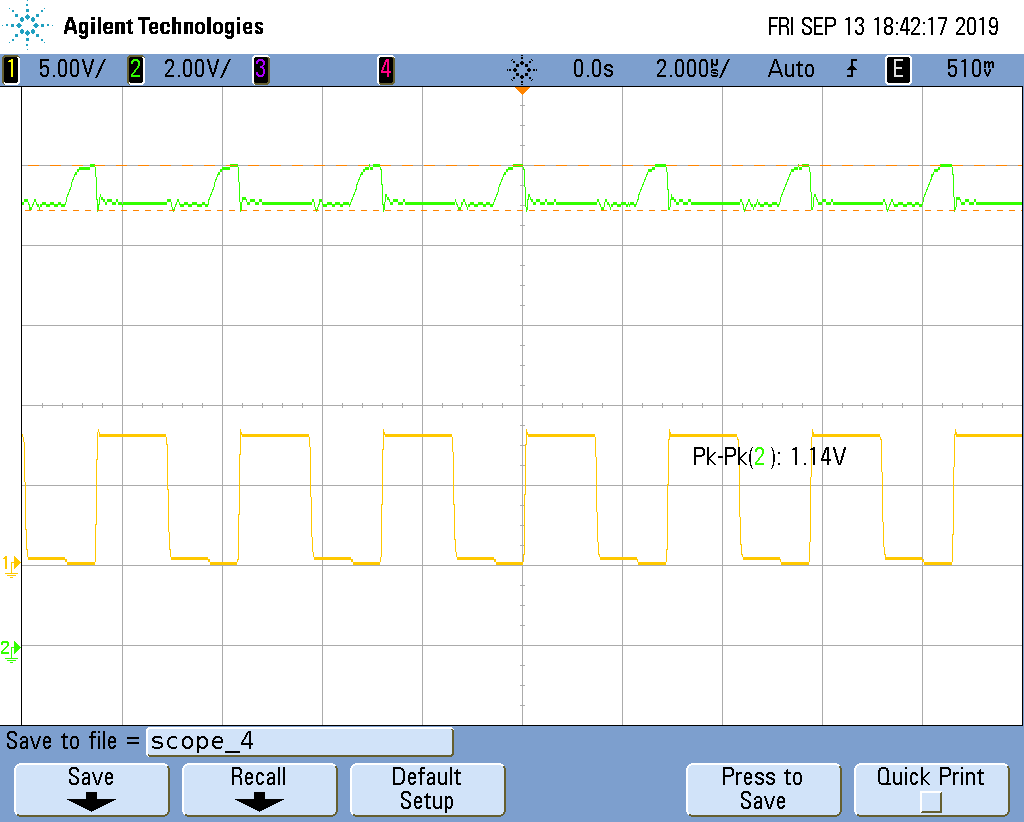
\includegraphics[scale=0.2]{../Mediciones/Osciloscopio/Barrido_Frecuencia/scope_4.png} 
    \end{tabular}
    \caption{Mediciones variando la frecuencia de la entrada}
    \label{fig:barrido_frecuencia}
\end{figure}

\subsection{Barrido de duty}
Se excita al circuito configurando con el generador una onda cuadrada de frecuencia $f = 25kHz$, la amplitud se mantiene de igual forma que en el an\'alsis anterior y luego
se var\'ia el valor del duty cycle de la onda desde el $20\%$ hasta el $80\%$. Los resultados de cuatro de las mediciones realizadas se pueden observar en la Fig.
\ref{fig:barrido_duty}, donde si bien se puede observar de las propias mediciones, es necesario aclarar que la onda amarilla corresponde a la onda de entrada y luego la verda a la salida,
y respectivamente se configuraron con duty $20\%$, $40\%$, $50\%$ y $60\%$.

Se puede verificar que a medida que el duty aumenta, luego tambi\'en el nivel de continua a la salida lo hace, lo cual desde un punto de vista f\'isico tiene sentido ya que se aumenta el intervalo de tiempo
durante el cual el transistor entra en modo saturaci\'on y se carga el inductor, aumentando la cantidad de energ\'ia que luego esta contiene y entrega al capacitor, que en consecuencia se carga a un nivel de tensi\'on superior.
No obstante, si se realiza un an\'alisis te\'orico del circuito se puede encontrar que la expresi\'on matem\'atica que gobierna la relaci\'on entrada y salida respecto del valor del duty est\'a dada como se muestra en la Ec. \ref{eq:salida_duty},
lo cual no se puede verificar completamente en la pr\'actica, ya que para todas las mediciones realizadas siempre hay un error de aproximadamente $E_R \approx 20\%$, que de todas formas no permanece igual para todos los casos.

\begin{equation}
    H = \frac{V_o}{V_i} = \frac{1}{1 - D}
    \label{eq:salida_duty}
\end{equation}

\begin{figure}[H]
    \centering
    \begin{tabular}{c c}
        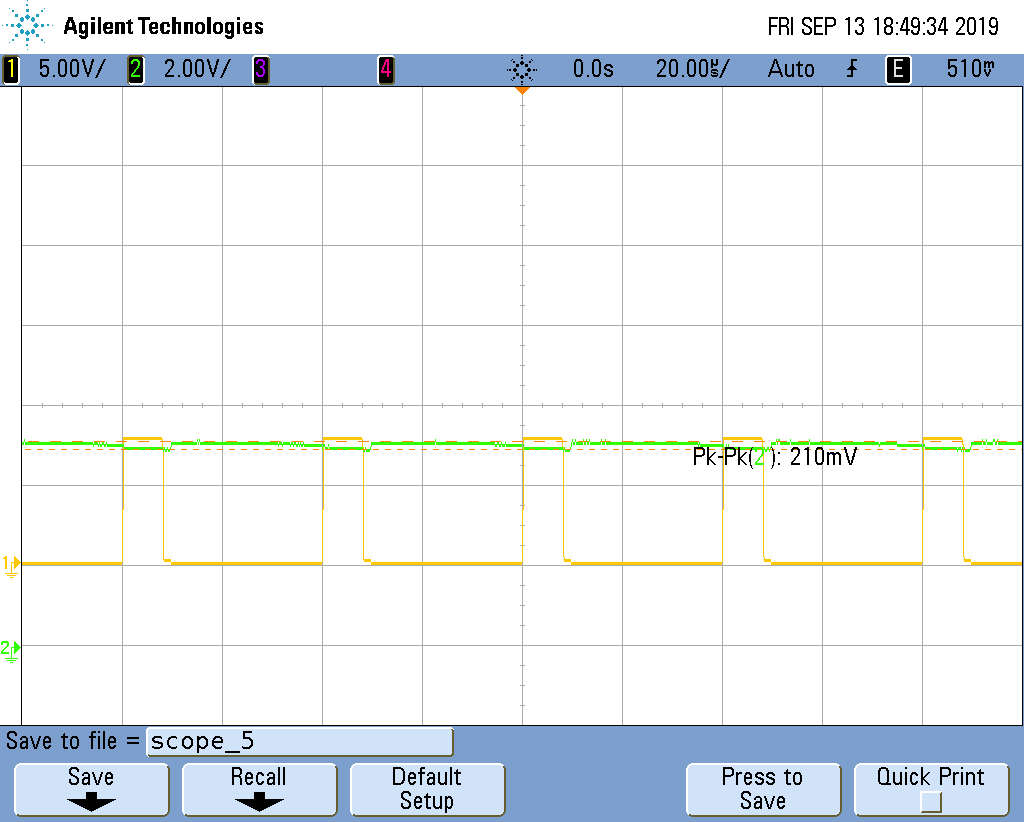
\includegraphics[scale=0.2]{../Mediciones/Osciloscopio/Barrido_Duty/scope_5.png} & 
        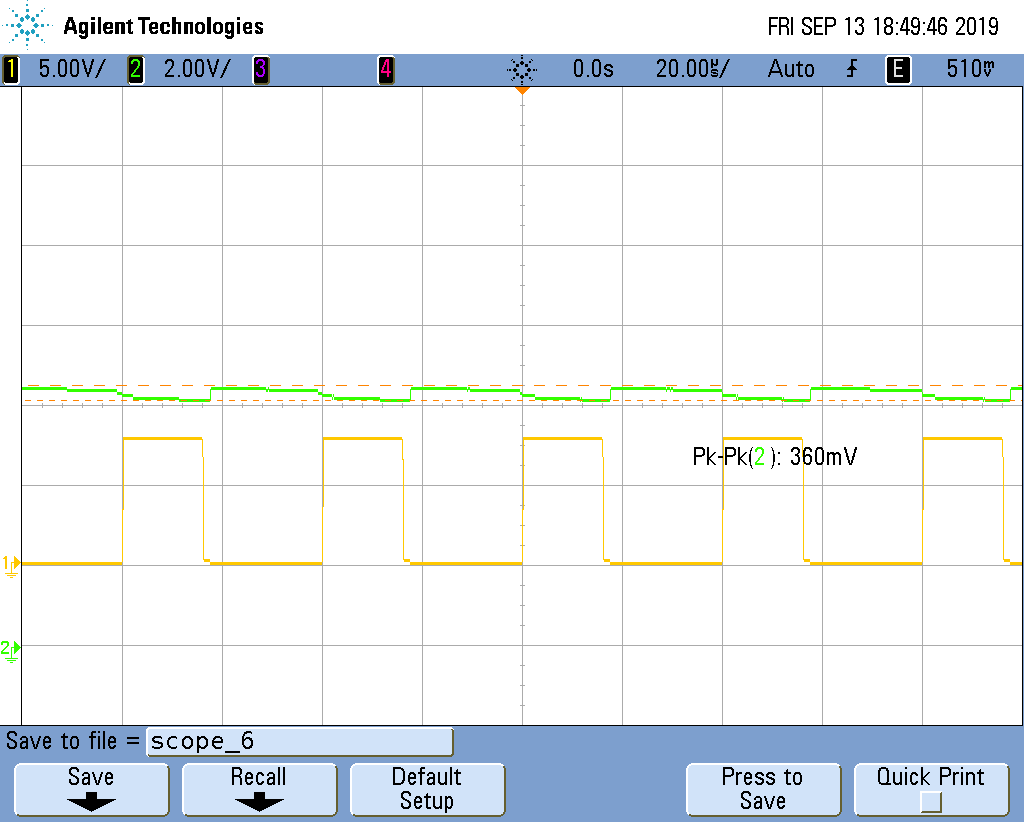
\includegraphics[scale=0.2]{../Mediciones/Osciloscopio/Barrido_Duty/scope_6.png} \\
        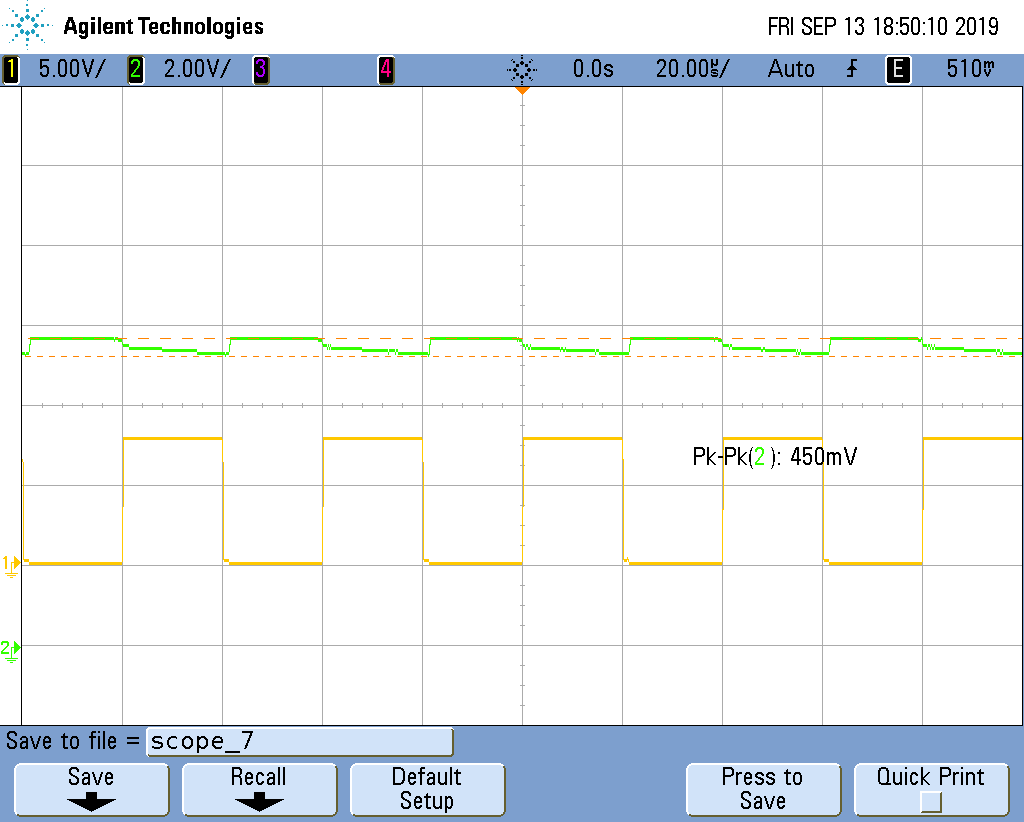
\includegraphics[scale=0.2]{../Mediciones/Osciloscopio/Barrido_Duty/scope_7.png} & 
        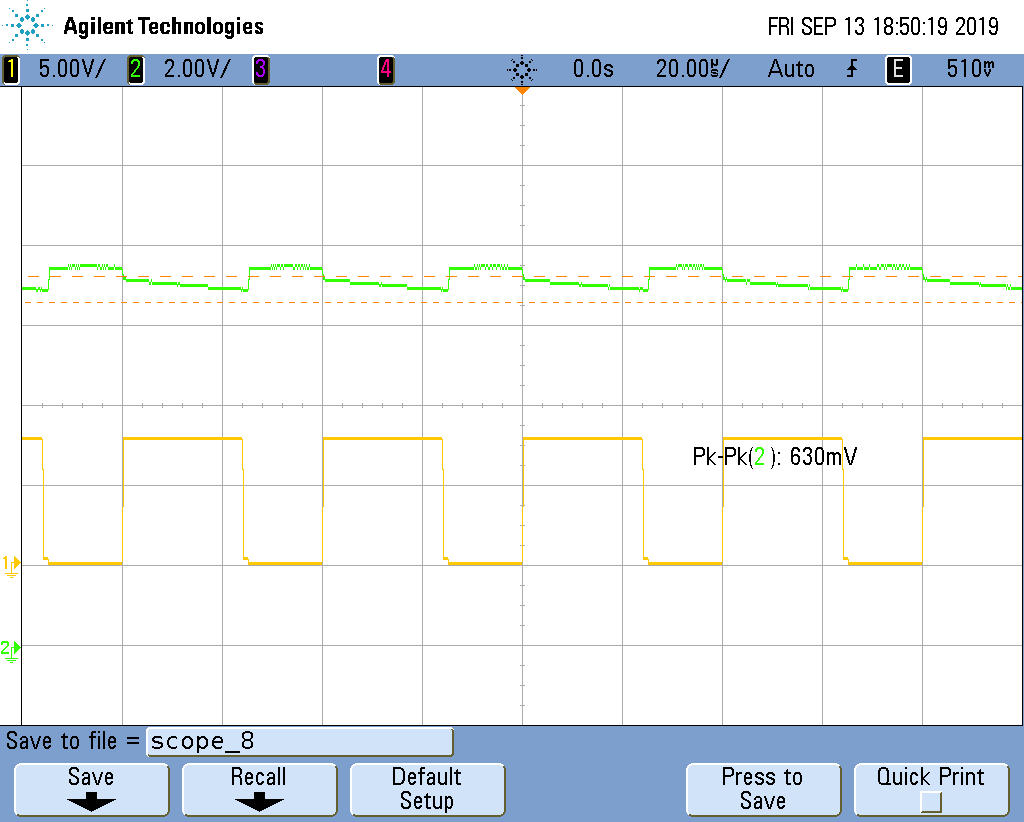
\includegraphics[scale=0.2]{../Mediciones/Osciloscopio/Barrido_Duty/scope_8.png} \\
    \end{tabular}
    \caption{Mediciones variando el duty de la entrada}
    \label{fig:barrido_duty}
\end{figure}

\subsection{Respuesta al escal\'on}
Establenciendo que las condiciones nominales de la operaci\'on del circuito es utilizando como excitaci\'on en la entrada del transistor una onda cuadrada de $f = 25kHz$ y $D = 50\%$, luego se configura el osciloscopio en modo Single y desconectando
y conectando la fuente de alimentaci\'on $V_d$ del circuito, se mide la respuesta al escal\'on del convertidor boost. La forma de onda resultante se puede observar en la Fig. \ref{fig:respuesta_escalon} de lo que puede deducirse un comportamiento
de segundo orden en estado subamortiguado que luego de un tiempo alcanza a establerse en el r\'egimen permanente, y a lo largo de todo ese proceso alcanzan a verse las variaciones producidas por la conmutaci\'on del transistor.

\begin{figure}[H]
    \centering
    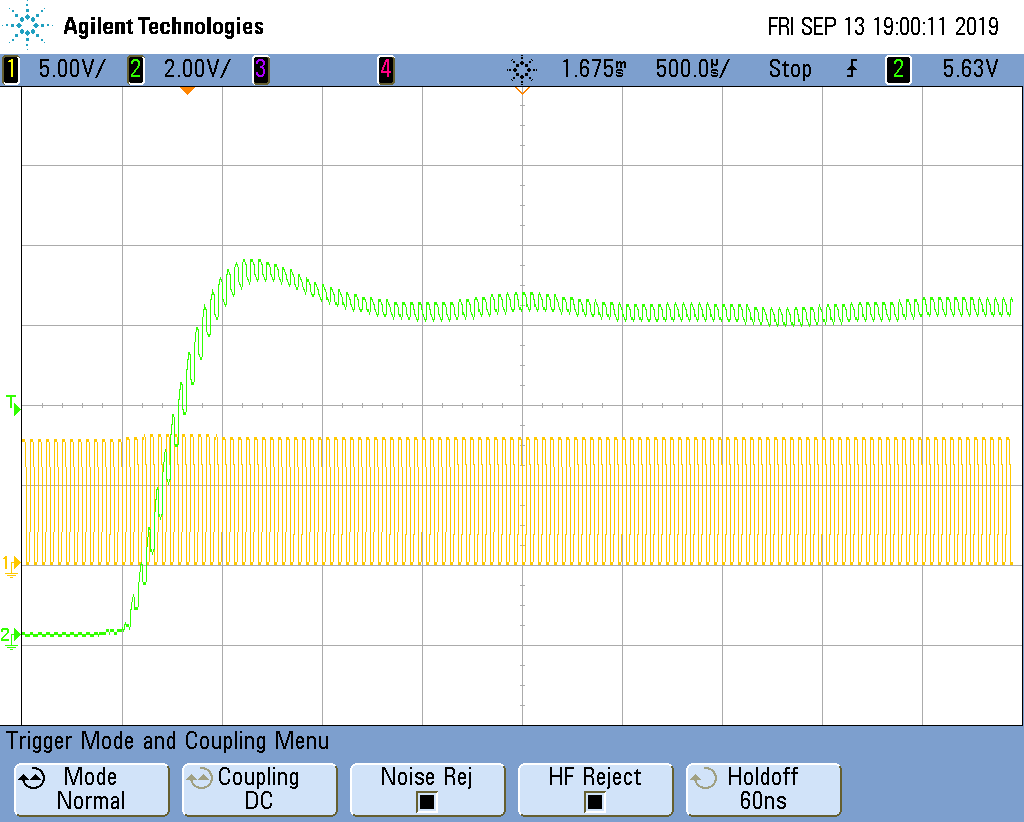
\includegraphics[scale=0.4]{../Mediciones/Osciloscopio/Respuesta_Escalon/scope_13.png}
    \caption{Medici\'on de la respuesta al escal\'on del Convertidor Boost}
    \label{fig:respuesta_escalon}
\end{figure}

\subsection{Medici\'on de ripple}
En la primera de las mediciones presentadas en este trabajo se pudo observar el ripple de la salida para el caso del circuito propuesto, con lo cual ahora se busca comparar el resultado cuando se agrega
a la salida otro capacitor de valor $100nF$ particularmente de tecnolog\'ia cer\'amico multicapa. El objetivo de esto no es s\'olo aumentar la capacidad para reducir las variaciones de ripple por mantener mayor cargas, sino que adem\'as
al tener varios capacitores en la salida de diversas tecnolog\'ias se logra mejorar el comportamiento de los mismos compensando algunos de sus efectos.

En la figura, la medici\'on de la izquierda corresponde al caso donde \'unicamente se tiene un capacitor electrol\'itico, mientras que en la de la derecha se agreg\'o un capacitor cer\'amico.

\begin{figure}[H]
    \centering
    \begin{tabular}{c c}
        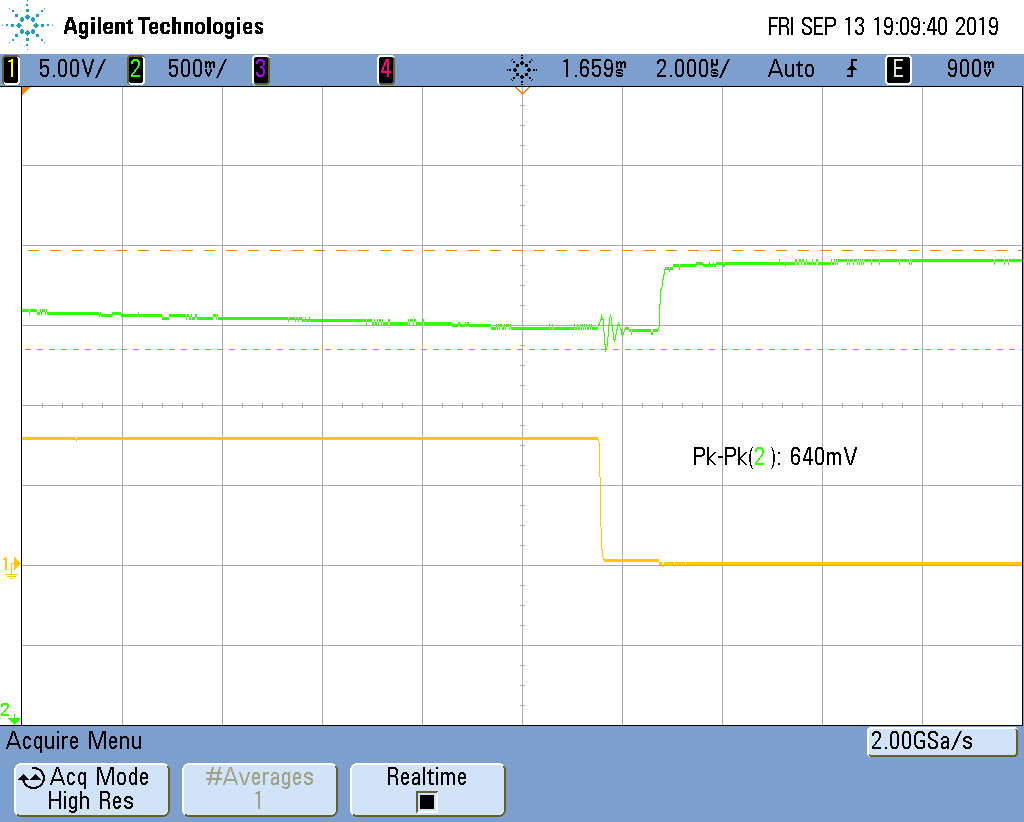
\includegraphics[scale=0.2]{../Mediciones/Osciloscopio/Ripple_Capacitor_Adicional/scope_15.png} &
        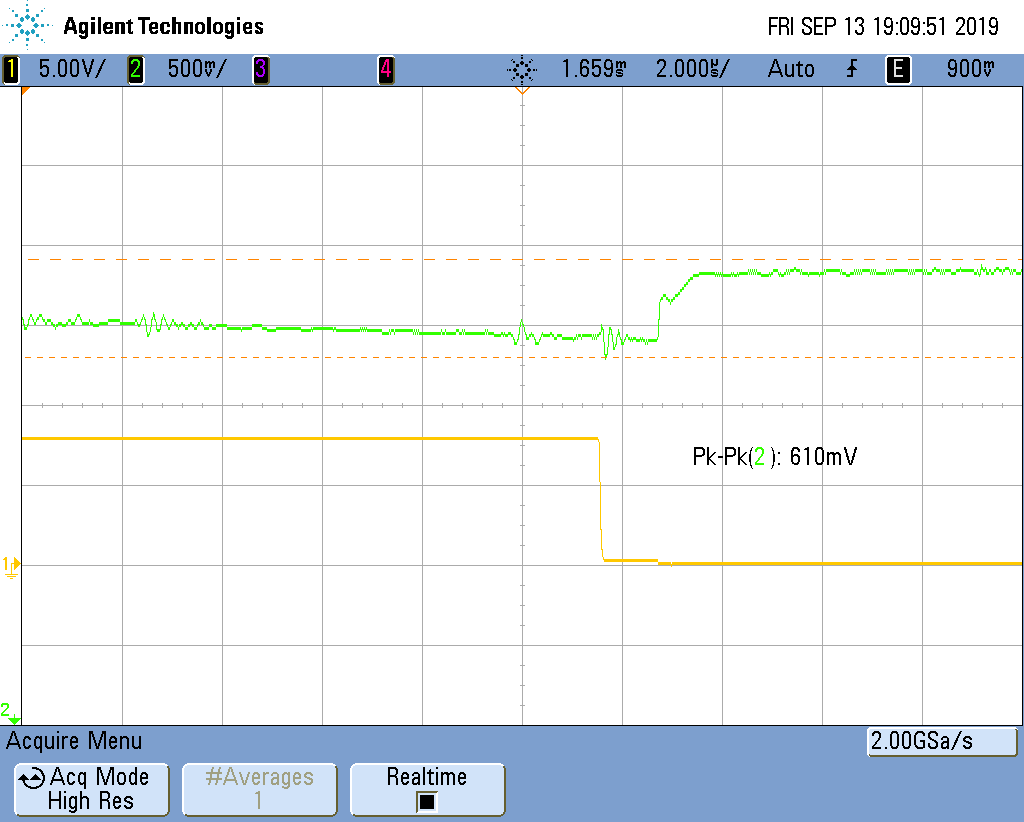
\includegraphics[scale=0.2]{../Mediciones/Osciloscopio/Ripple_Capacitor_Adicional/scope_16.png}  
    \end{tabular}
    \caption{Medici\'on del ripple de la salida}
    \label{fig:salida_ripple}
\end{figure}

En la Fig. \ref{fig:circuito_equivalente} se puede observar el circuito inicialmente propuesto con un capacitor de salida adicional que es el que se describi\'o previamente como cer\'amico de $100nF$. Adem\'as,
se reemplazaron los capacitores por sus modelos paralelos en su forma m\'as simple, esto es, considerando \'unicamente una resistencia en paralelo correspondiente a las corrientes de p\'erdida a trav\'es del diel\'ectrico del capacitor,
sin considerar otros efectos como inductancias o resistencias par\'asitas por los terminales o por los procesos de fabricaci\'on como suele ser en el caso del electrol\'itico por el enrollado de las l\'aminas de material conductor y aislante.
Las diferencias constructivas de las tecnolog\'ias de ambos capacitores suelen resultar en diferentes caracter\'isticas como el orden de magnitud de las resistencias en paralelo o bien el rango de operaci\'on para la frecuencia, con lo cual
emplear un banco de diferentes tecnolog\'ias permite compensar para las regiones en las cuales algunas de ellas no tienen un buen rendimiento, con otras que s\'i lo tienen. No obstante, sigue requiriendose un capacitor electrol\'itico por su alto valor de capacidad
frente al caso del cer\'amico.

\begin{figure}[H]
    \centering
    \includegraphics[scale=0.45]{Recursos/circuito_con_equivalentes.png}
    \caption{Circuito con capacitor adicional y modelos del mismo}
    \label{fig:circuito_equivalente}
\end{figure}

\subsection{Caracterizaci\'on de la bobina L}
Se busca caracterizar el estado de la bobina L durante el funcionamiento de circuito, para ello se mide su tensi\'on y corriente, adem\'as de determinar su valor de forma emp\'irica. Para lograr esto,
en primer lugar se mide la tensi\'on en el colector del transistor y luego sobre la tensi\'on de la fuente de alimentaci\'on, finalmente se emplea la funci\'on del osciloscopio para obtener la diferencia.
Por otro lado, para obtener la corriente se agreg\'o una resistencia en serie de un valor de $R = 10\Omega$ sobre la cual se repiti\'o el proceso.
Finalmente, con estas mediciones se puede determinar el valor de corriente y tensi\'on del inductor en funci\'on del tiempo. Para obtener el valor de la inductancia se integra la tensi\'on obtenida sobre el inductor
y la tensi\'on obtenida sobre la resistencia auxiliar que se utiliz\'o para medir la corriente, de forma tal que existe una relaci\'on proporcional en funci\'on la de inductancia entre tales magnitudes.

Cabe mencionar que, en la captura de la izquierda, la se\~nal de color amarilla es la tens\'on en el colector del trasistor, luego la de color violeta corresponde a la funci\'on math que es la integral de la diferencia de potencial sobre la bobina, y finalmente
la verde corresponde a la tensi\'on antes de la bobina.
En la captura de la derecha, la se\~nal verde y la amarilla corresponden a la tensi\'on antes y despues de la resistencia y  violeta corresponde a la diferencia de ambos canales, lo cual permite medir la caida de tensi\'on en la resistencia. 

\begin{figure}[H]
    \centering
    \begin{tabular}{c c}
        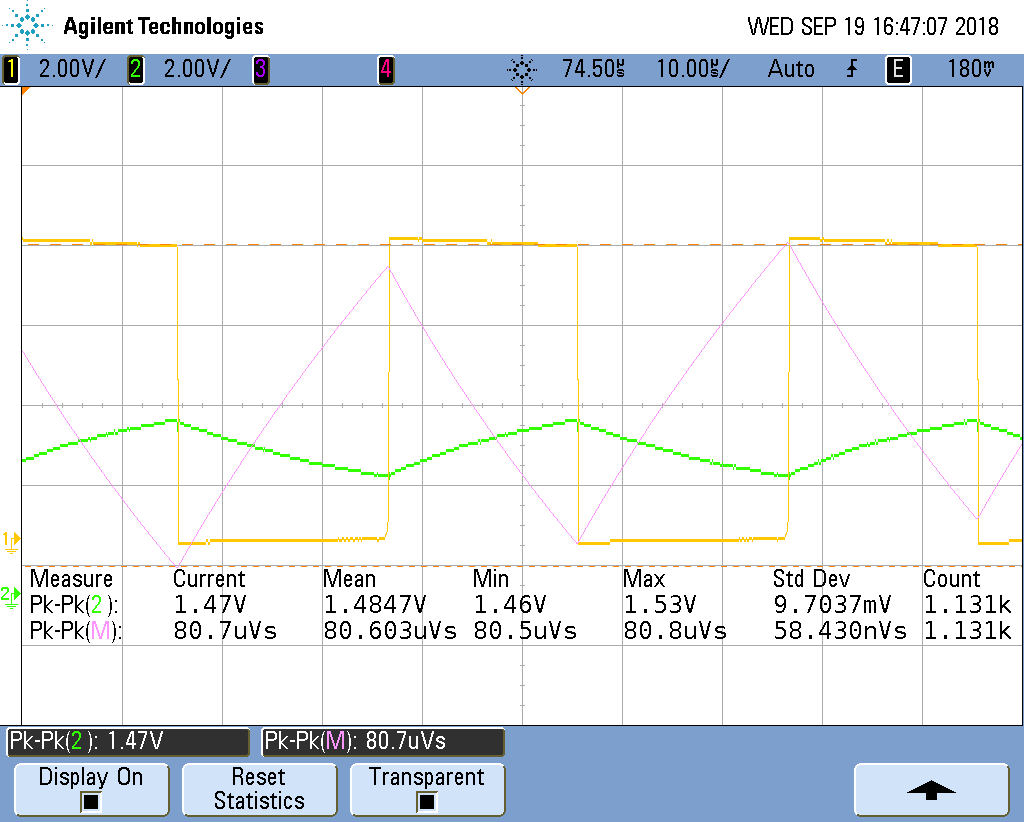
\includegraphics[scale=0.2]{../Mediciones/int_vl.png} &
        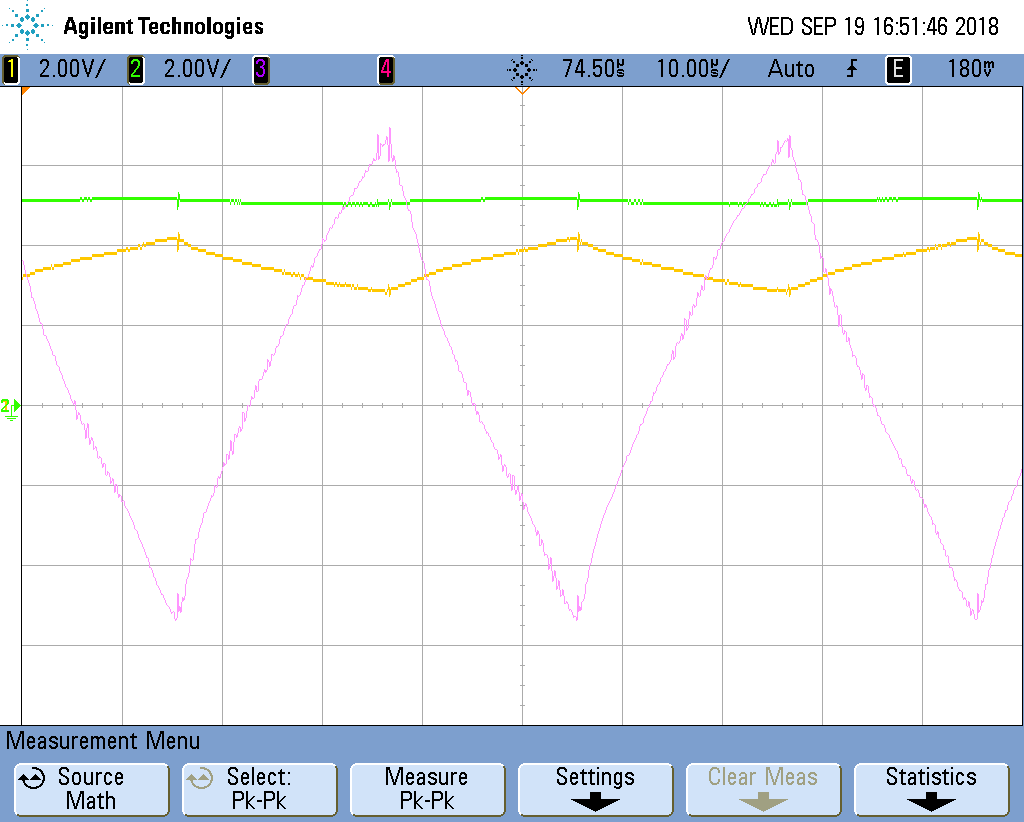
\includegraphics[scale=0.2]{../Mediciones/VR_Limpio.png}  
    \end{tabular}
        \caption{Mediciones sobre la  tensi\'on sobre el inductor y la resistencia}
    \label{fig:mediciones_inductor}
\end{figure}

Para determinar a partir de los datos obtenidos el valor de la inductancia L, entonces se plantea:

\begin{align*}
    & V_L(t) = L \cdot \frac{\delta i_L(t)}{\delta t} \\
    & \int V_L(t) \cdot \delta t = L \cdot i_L(t) \\
    & \int V_L(t) \cdot \delta t = \frac{L}{R_{aux}} \cdot V_R(t) \\
    & \Rightarrow L = \frac{\int V_L(t) \cdot \delta t}{V_R(t)} \cdot R_{aux} \\
    & \Rightarrow L = 548.97\mu \Omega
\end{align*}

\subsection{Caracterizaci\'on del transistor Q1}
\label{sec:TBJ_Q1}
Se muestra en esta secci\'on las mediciones realizadas sobre la base $(V_{BE})$ y colector$(V_{CE})$ del transistor. Se muestra en la Figura \ref{fig:vce_vbe} la captura de pantalla tomada del osciloscopio. Estas mediciones se realizan con el generador de onda cuadrada conectado a la base del transistor con una frecuencia $f = 25KHz$ y un duty cycle $D = 50\%$.

\begin{figure}[H]
    \centering
    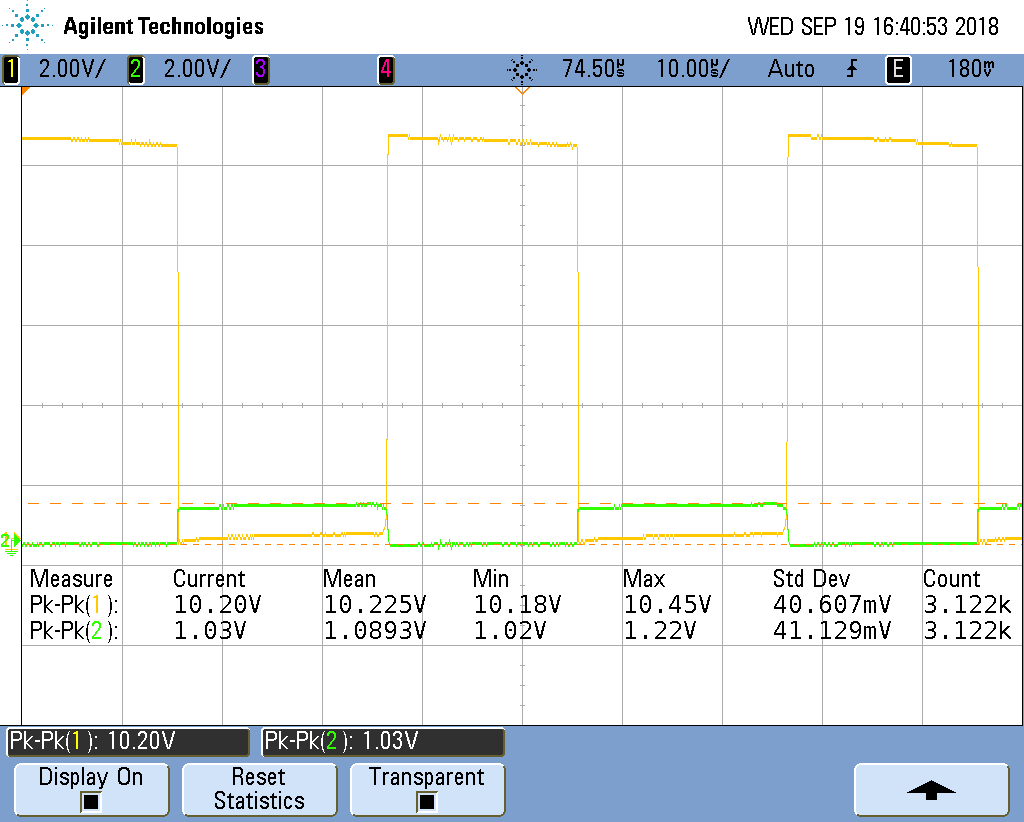
\includegraphics[scale=0.4]{../Mediciones/f.png}
    \caption{Mediciones de $V_{BE}(Verde)$ y $V_{CE}(Amarillo)$del transistor}
    \label{fig:vce_vbe}
\end{figure}
Se pueden observar claramente las 2 regiones de inter\'es, el corte y la saturac\'ion del transistor.
Cuando la se\~nal cuadrada en la base es $0V$ y $V_{BE} = 0V$ la juntura base-emisor no se polariza y  el transistor se comporta como un circuito abierto (corte). Por consiguiente, $V_{CE} \simeq V_o - V_D$ siendo $V_D$ la tensi\'on que cae en el diodo de aproximadamente $0.7V$.
Cuando el transistor se encuentra en saturaci\'on, en cambio, se puede observar que la juntura base-emisor se polariza en directa, por lo que $V_{BE} \simeq 1V$ y $V_{CE} \simeq 0V$. Esto sucede cuando la se\~nal de entrada es de $5V$


\subsection{Caracterizaci\'on del transistor Q1 con accesorio resorte}
En esta secci\'on se busca comparar las mediciones realizadas con el accesorio resorte en la punta, con las realizadas conectando la masa de la punta con el cable, como se hace normalmente.Para realizar dichas mediciones por se conserva la configuraci\'on utilizada en la secci\'on anterior.
Se muestra en la Figura \ref{fig:c/s_res} los resultados obtenidos.
\begin{figure}[H]
    \centering
    \begin{tabular}{c c}
        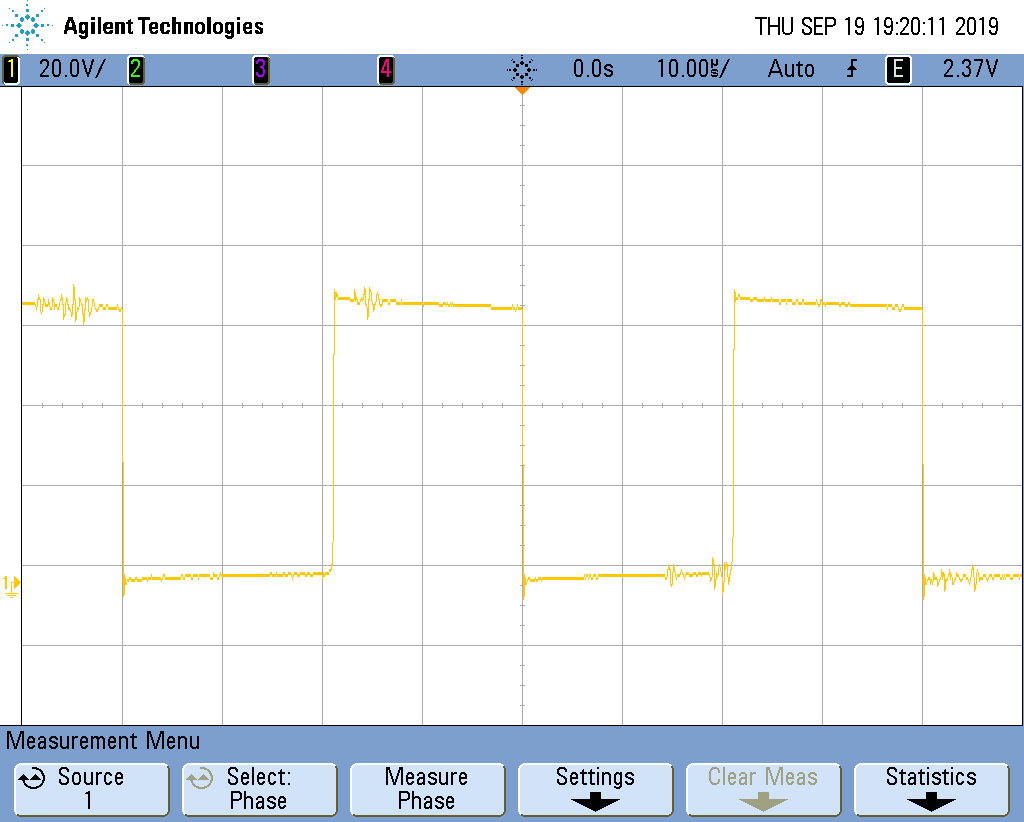
\includegraphics[scale=0.2]{../Mediciones/scope_2.png} &
        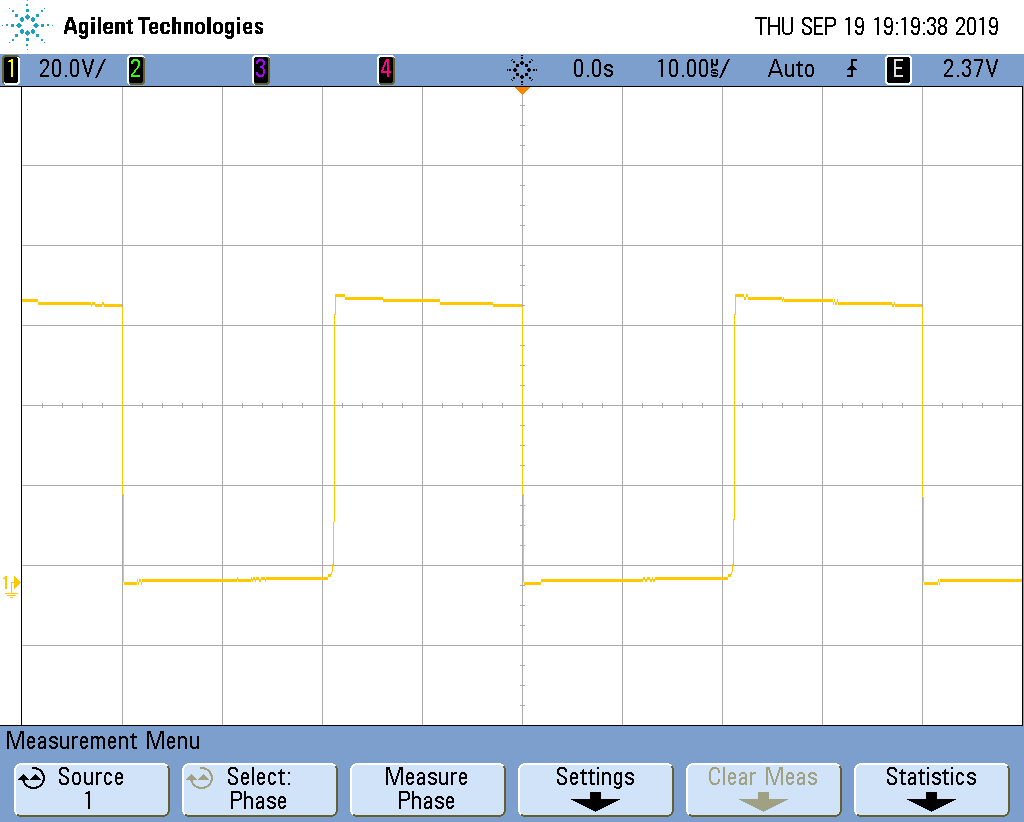
\includegraphics[scale=0.2]{../Mediciones/scope_0.png}  
    \end{tabular}
    \caption{Medici\'on del $V_{CE}$ sin resorte (Izquerda) y con resorte (Derecha)}
    \label{fig:c/s_res}

\end{figure}
Si bien en las capturas del osciloscopio solo se toma el trazo de una pasada del haz digital, lo que hace que la diferencia no sea tan notable, se puede ver como el ruido inducido en la medici\'on de la manera usual hace que la se\~nal se deforme. Este efecto es mucho menos notorio, por no decir casi inexistente, en la medici\'on realizada con el accesorio resorte.  
\end{document}
